\documentclass{mwhittaker}
\title{Bipartisan Paxos}

\usepackage{appendix}
\usepackage{mdframed}
\usepackage{multirow}
\usepackage{pervasives}
\usepackage{subcaption}
\usepackage{tikz}
\usetikzlibrary{calc}
\usetikzlibrary{positioning}
\usetikzlibrary{shapes.misc}

\theoremstyle{definition}
\newmdtheoremenv[innertopmargin=0pt]{boxedinvariant}{Invariant}

\newcommand{\deps}[1]{\text{deps}(#1)}

\begin{document}
\maketitle

\begin{abstract}
  Egalitarian Paxos~\cite{moraru2013there}, or EPaxos, is a state machine
  replication protocol like Raft~\cite{ongaro2014search} or Viewstamped
  Replication~\cite{liskov2012viewstamped}. EPaxos has a number of nice features
  that set it apart from other state machine replication protocols. For example,
  it can choose non-conflicting commands in one round trip, disjoint sets of
  conflicting commands do not affect each other, and superquorum sizes are one
  node smaller than the superquorum sizes used by other protocols.
  %
  In this paper, we describe a family of consensus algorithms that are derived
  from EPaxos. We call them Bipartisan Paxos, Unanimous Bipartisan Paxos, and
  Fast Bipartisan Paxos.
\end{abstract}

\section{Bipartisan Paxos}\seclabel{BipartisanPaxos}
In this section, we describe \defword{Bipartisan Paxos}, or \defword{BPaxos}.
BPaxos is designed to be as simple to understand as possible, even at the cost
of performance. Other variants of BPaxos that we'll see later (i.e.\ Unanimous
BPaxos and Fast BPaxos) improve on BPaxos' performance.

\paragraph{Overview}
MultiPaxos allows a set of nodes to agree on a totally ordered sequence of
state machine commands. This is illustrated in \figref{MultiPaxosCartoon}.

\tikzstyle{square}=[%
  draw,
  line width=1pt,
  minimum height=0.5in,
  minimum width=0.5in,
  text width=0.4in,
  align=center
]
\begin{figure}[h]
  \centering
  \begin{tikzpicture}
    \node[square] (a) at (0, 0) {\texttt{x=1}};
    \node[square, right=-1pt of a] (b) {\texttt{y=1}};
    \node[square, right=-1pt of b] (c) {\texttt{y+=x}};
    \node[square, right=-1pt of c] (d) {\texttt{y+=1}};
    \node[square, right=-1pt of d] (e) {\texttt{x=2\\y=2}};
    \node[square, right=-1pt of e] (f) {};
    \node[square, right=-1pt of f] (g) {};
    \node[right=0in of g] (h) {\ldots};

    \foreach \label/\i in {a/0, b/1, c/2, d/3, e/4, f/5, g/6} {%
      \node[below=0in of \label] {\i};
    }
  \end{tikzpicture}
  \caption{MultiPaxos}\figlabel{MultiPaxosCartoon}
\end{figure}

While simple, agreeing on a totally ordered sequence of state machine commands
can be overly prescriptive. If two commands conflict (e.g., \texttt{x = 1} and
\texttt{x = 2}), then they \emph{do} need to be executed by every state machine
replica in the same order. But, if two commands do \emph{not} conflict (e.g.,
\texttt{x = 1} and \texttt{y = 1}), then they do \emph{not} need to be totally
ordered.  State machine replicas can execute them in either order.

EPaxos takes advantage of this fact and attempts to order commands only if they
conflict. To do so, it ditches the totally ordered sequence and instead agrees
on a directed graph of commands such that every pair of conflicting commands
have an edge between them. An example is illustrated in \figref{EPaxosCartoon}%
\footnote{%
  In reality, the graph would be the transitive closure of the one in
  \figref{EPaxosCartoon}, but we do not draw all edges to keep things simple
}.
EPaxos then executes this graph in reverse topological order one strongly
connected component at a time, executing commands within a component in an
arbitrary but deterministic order. For example, in \figref{EPaxosCartoon}, we
could execute commands in the order $R.1, R.2, S.1, Q.2, Q.1$.

\begin{figure}[h]
  \centering
  \begin{tikzpicture}[scale=2.5]
    \node[square] (a) at (0, 1) {\texttt{x=1}};
    \node[square] (b) at (0, 0) {\texttt{y=1}};
    \node[square] (c) at (1, 1) {\texttt{y+=x}};
    \node[square] (d) at (1, 0) {\texttt{y+=1}};
    \node[square] (e) at (2, 0.5) {\texttt{x=2\\y=2}};
    \draw[ultra thick, -latex] (c) to (a);
    \draw[ultra thick, -latex] (c) to (b);
    \draw[ultra thick, -latex, bend right] (c) to (e);
    \draw[ultra thick, -latex] (d) to (b);
    \draw[ultra thick, -latex, bend right] (e) to (c);
    \draw[ultra thick, -latex] (e) to (d);

    \foreach \label/\i in {a/$R.1$, b/$R.2$, c/$Q.1$, d/$S.1$, e/$Q.2$} {%
      \node[above=0in of \label] {\i};
    }
  \end{tikzpicture}
  \caption{EPaxos}\figlabel{EPaxosCartoon}
\end{figure}

Every vertex in the graph has a unique name like $Q.1$ or $R.1$. EPaxos calls
these \defword{instances}. We can view a named vertex, the command inside the
vertex, and the vertex's outbound edges as a little gadget. For example,
\figref{EPaxosGadgets} shows gadgets for vertices $R.2$, $Q.1$, and $Q.2$.
%
More formally, we can think of these gadgets as tuples like $(Q.1,
\texttt{y+=x}, \set{R.1, R.2, Q.2})$ where $Q.1$ is the name of the vertex,
\texttt{y+=x} is the command inside the vertex, and the set $\set{R.1, R.2,
Q.2}$ is the set of \defword{dependencies} of $Q.1$ (or of \texttt{y+=x} if
$Q.1$ is clear from context).

\begin{figure}[h]
  \centering

  \begin{subfigure}[b]{0.19\textwidth}
    \begin{tikzpicture}[scale=2.5]
      \node[square] (b) at (0, 0) {\texttt{y=1}};
      \foreach \label/\i in {b/$R.2$} {%
        \node[above=0in of \label] {\i};
      }
    \end{tikzpicture}
  \end{subfigure}
  %
  \begin{subfigure}[b]{0.49\textwidth}
    \begin{tikzpicture}[scale=2.5]
      \node[square] (a) at (0, 1) {};
      \node[square] (b) at (0, 0) {};
      \node[square] (c) at (1, 1) {\texttt{y+=x}};
      \node[square] (e) at (2, 0.5) {};
      \draw[ultra thick, -latex] (c) to (a);
      \draw[ultra thick, -latex] (c) to (b);
      \draw[ultra thick, -latex, bend right] (c) to (e);
      \foreach \label/\i in {a/$R.1$, b/$R.2$, c/$Q.1$, e/$Q.2$} {%
        \node[above=0in of \label] {\i};
      }
    \end{tikzpicture}
  \end{subfigure}
  %
  \begin{subfigure}[b]{0.29\textwidth}
    \begin{tikzpicture}[scale=2.5]
      \node[square] (c) at (1, 1) {};
      \node[square] (d) at (1, 0) {};
      \node[square] (e) at (2, 0.5) {\texttt{x=2\\y=2}};
      \draw[ultra thick, -latex, bend right] (e) to (c);
      \draw[ultra thick, -latex] (e) to (d);
      \foreach \label/\i in {c/$Q.1$, d/$S.1$, e/$Q.2$} {%
        \node[above=0in of \label] {\i};
      }
    \end{tikzpicture}
  \end{subfigure}

  \caption{EPaxos Gadgets}\figlabel{EPaxosGadgets}
\end{figure}

EPaxos nodes collectively construct the directed graph of commands by stitching
together a bunch of gadgets. An EPaxos node $R$ proposes a gadget for instance
$R.i$ and attempts to get the gadget chosen. Once a gadget is chosen, it is
considered part of the directed graph and is eligible for execution. EPaxos'
correctness hinges on the following two key invariants.

\begin{boxedinvariant}\label{inv:GadgetsChosen}
  Once a gadget $(R.i, a, \deps{a})$ has been chosen, no other gadget can be
  chosen for instance $R.i$.
\end{boxedinvariant}

\begin{boxedinvariant}\label{inv:ConflictingGadgets}
  If two gadgets $(I_a, a, \deps{a})$ and $(I_b, b, \deps{b})$ are chosen and
  commands $a$ and $b$ conflict, then either $I_a \in \deps{b}$ or $I_b \in
  \deps{a}$ or both.
\end{boxedinvariant}

BPaxos, like EPaxos, also constructs a directed graph of commands and executes
them in reverse topological order one strongly connected component at a time.
In fact, BPaxos and EPaxos execute commands in 100\% the same way. BPaxos also
maintains the same two key invariants as EPaxos. BPaxos and EPaxos differ only
in how they construct the directed graph of commands.
%
BPaxos is illustrated in \figref{BPaxos}. A BPaxos instance has three main
components: an ordering service, a consensus service, and a set of BPaxos
nodes. We now explain these three components.

{\begin{figure}[ht]
  \centering

  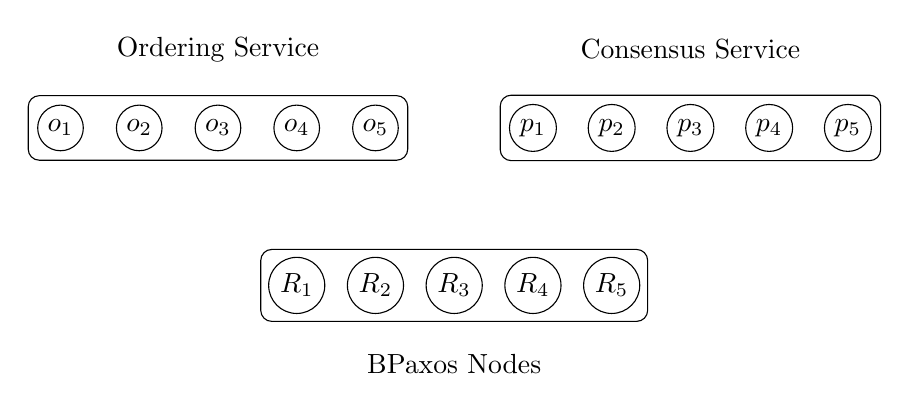
\begin{tikzpicture}
    \tikzstyle{machine}=[draw, circle, inner sep=2pt]

    % Ordering Service
    \node[machine] (o1) at (0, 2) {$o_1$};
    \node[machine] (o2) at (1, 2) {$o_2$};
    \node[machine] (o3) at (2, 2) {$o_3$};
    \node[machine] (o4) at (3, 2) {$o_4$};
    \node[machine] (o5) at (4, 2) {$o_5$};
    \node (os) at (2, 3) {Ordering Service};
    \draw[rounded corners]
      ($(o1.south west) + (-0.2, -0.2)$) rectangle
      ($(o5.north east) + (0.2, 0.2)$);

    % Consensus
    \node[machine] (p1) at (6, 2) {$p_1$};
    \node[machine] (p2) at (7, 2) {$p_2$};
    \node[machine] (p3) at (8, 2) {$p_3$};
    \node[machine] (p4) at (9, 2) {$p_4$};
    \node[machine] (p5) at (10, 2) {$p_5$};
    \node (os) at (8, 3) {Consensus Service};
    \draw[rounded corners]
      ($(p1.south west) + (-0.2, -0.2)$) rectangle
      ($(p5.north east) + (0.2, 0.2)$);

    % BPaxos Nodes
    \node[machine] (b1) at (3, 0) {$R_1$};
    \node[machine] (b2) at (4, 0) {$R_2$};
    \node[machine] (b3) at (5, 0) {$R_3$};
    \node[machine] (b4) at (6, 0) {$R_4$};
    \node[machine] (b5) at (7, 0) {$R_5$};
    \draw[rounded corners]
      ($(b1.south west) + (-0.2, -0.2)$) rectangle
      ($(b5.north east) + (0.2, 0.2)$);
    \node (bpaxos) at (5, -1) {BPaxos Nodes};
  \end{tikzpicture}

  \caption{BPaxos}\figlabel{BPaxos}
\end{figure}
}

TODO: revise ordering service now that we have the two main invariants.

\paragraph{Ordering Service}

The ordering service is responsible for computing the dependencies between
conflicting state machine commands. When a BPaxos node $R$ receives a state
machine command $a$ from a client, it chooses some instance $R.i$ for $a$.
Then, $R$ sends $a$ and $R.i$ to the ordering service. When the ordering
service receives a command $a$ for instance $R.i$, it replies with a tuple $(a,
R.i, \deps{a})$ where $\deps{a} = \set{I_1, \ldots, I_n}$ is a set of instances
that we call $a$'s \defword{dependencies}.

The ordering service provides the following guarantee. If two conflicting
commands $a$ and $b$ in instances $I_a$ and $I_b$ yield responses $(a,
\deps{a})$ and $(b, \deps{b})$ from the ordering service, then either $I_a \in
\deps{b}$ or $I_b \in \deps{a}$ (or both). That is, if two conflicting commands
are sent to the ordering service, at least one is guaranteed to be a dependency
of the other.

Note that the ordering service makes the following assumption. At most one
command can be sent in any given instance. BPaxos satisfies this invariant
because $R$ assigns every command $a$ to a unique instance $R.i$, and no other
EPaxos node contacts the ordering service for an instance $R.i$.

Implementing a fault tolerant ordering service is straightforward. We employ
$2f + 1$ ordering service nodes $o_{1}, \ldots, o_{2f + 1}$. When a BPaxos node
$R$ sends a command $a$ in instance $R.i$ to the ordering service, it sends the
command to all $2f + 1$ of the ordering service nodes. Every ordering service
node $o_i$ maintains a set $O_i = {(c_1, I_1), (c_2, I_2), \ldots}$ of all the
commands and corresponding instances that it has received. When node $o_i$
receives a command $a$ for instance $R.i$ from a BPaxos node, it atomically
performs two actions.
\begin{enumerate}
  \item
    $o_i$ replies to $R$ with the tuple $(a, R.i, \deps{a}_i)$ where
    $\deps{a}_i$ is the set of instances $I$ for which there exists a $(c, I)
    \in O_i$ such that $a$ and $c$ conflict. This is the set of instances that
    $o_i$ has previously received that contain a command that conflict with
    $a$.

  \item
    $o_i$ adds $(a, R.i)$ to $O_i$.
\end{enumerate}

When a BPaxos node receives replies $(a, R.i, \deps{a}_{i_1}), \ldots, (a, R.i,
\deps{a}_{i_{f+1}})$ from a quorum $Q_a$ of $f + 1$ ordering service nodes, it
takes $(a, R.i, \deps{a}_{i_1} \cup \ldots \cup \deps{a}_{i_{f+1}}) = (a,
\deps{a})$ to be the response from the ordering service.

To understand why this ordering service implementation provides its advertised
guarantees, consider conflicting commands $a$ and $b$ in instances $I_a$ and
$I_b$. Assume $a$'s reply $(a, I_a, \deps{a})$ was formed from a quorum $Q_a$
and $b$'s reply $(b, I_b, \deps{b})$ was formed from a quorum $Q_b$. Any two
quorums intersect, so $Q_a \cap Q_b$ is nonempty. Let $o_i$ be an ordering
service node in this intersection. $o_i$ either received $a$ or $b$ first. If
it received $a$ first, then $(a, I_a)$ is in $O_i$ when $o_i$ processed command
$b$, so $o_i$ includes $I_a$ in $\deps{b}_i$, so $I_a$ is in $\deps{b}$.
Symmetrically, if $o_i$ received $b$ first, then it includes $I_b$ in
$\deps{a}$.

\paragraph{Consensus Service}
We assume we have some set $p_1, \ldots, p_n$ of nodes that implement Plain
Jane consensus. A BPaxos node can propose to the consensus service that some
value $v$ be chosen in some instance $I$. The consensus service replies with
the value that has been chosen in instance $I$, which may or may not be $v$
depending on if there are concurrent proposers proposing to instance $i$. The
consensus service guarantees that for every instance $i$, at most one value is
ever chosen in $i$.

We can implement the consensus service with one Paxos instance for every BPaxos
instance, with consensus service nodes playing the role of Paxos acceptors and
the BPaxos nodes playing the role of Paxos proposers. Similar to MultiPaxos, we
can have each EPaxos node $R$ serve as the leader for every Paxos instance
$R.i$. Initially, $R$ runs phase 1 of Paxos for every instance $R.i$, so that
later, $R$ can get a command committed in instance $R.i$ in one round trip to
the consensus service (in the best case).

\paragraph{BPaxos Nodes}
We assume a fixed set $R_1, \ldots, R_{2f+1}$ of $2f + 1$ BPaxos nodes.
%
Clients sends state machine commands to BPaxos nodes to be executed by the
replicated state machine. When a BPaxos node $R$ receives a command $a$, it
sends the command to the ordering service in a previously unused instance $R.i$
and receives a reply $(a, R.i, \deps{a})$. $R$ then proposes the value $(a,
\deps{a})$ to the consensus service in instance $R.i$. The consensus service
then replies with some chosen value $(a', \deps{a'})$ (which is equal to $(a,
\deps{a})$ in the failure-free case). At this point, the command $a'$ is
considered committed in instance $R.i$ of the directed graph of state machine
commands with outbound edges to instances in $\deps{a'}$. Node $R$ also informs
the other BPaxos nodes that the value $(a', \deps{a'})$ has been committed. As
noted earlier, the execution of the commands in the directed graph is identical
to that of EPaxos. Committed commands are executed in reverse topological
order, one strongly connected component at a time. Within a strongly connected
component, BPaxos executes commands in an arbitrary but deterministic order.
There are no sequence numbers, so BPaxos provides serializability instead of
linearizability. This is not fundamental. It just makes things a bit simpler.

\newcommand{\noop}{\text{noop}}
It's possible that (1) a committed command $a$ depends on an instance $R.i$
that contains an uncommitted command, and (2) the BPaxos node $R$ that manages
the instance $R.i$ has crashed. If the instance $R.i$ remains forever
uncommitted, then the command $a$ will never be executed. To avoid this
liveness violation, if any BPaxos node $S$ notices that instance $R.i$ has been
uncommitted for some time, it can propose to the consensus service that the
value $(\noop, \emptyset)$ be chosen in instance $R.i$ where $\noop$ is a
command that doesn't affect the state machine.

\paragraph{Correctness}
Now we prove that BPaxos is correct by leveraging EPaxos' proof of correctness.
Open up \cite{moraru2013proof} and head to section 5.6, which contains proofs
of EPaxos' correctness.
\begin{itemize}
  \item
    \textbf{Theorem 1} says that EPaxos satisfies nontriviality. Clearly, so
    does BPaxos.

  \item
    \textbf{Lemma 1} says that EPaxos commits a command in an instance only if
    no other command will ever be committed in the same instance. The fact that
    BPaxos satisfies Lemma 1 is immediate from the fact that we use a consensus
    service. In fact, Lemma 1 is really just a restatement of the exact
    property that the consensus service provides.

  \item
    \textbf{Theorem 2} follows from Lemma 1.

  \item
    \textbf{Theorem 3} is trivial.

  \item
    \textbf{Theorem 4} states that if two conflicting commands are both
    committed, then they will be executed in the same order by every BPaxos
    node. The proof that BPaxos satisfies Theorem 4 is more or less the same as
    the proof that EPaxos satisfies theorem 4, which shouldn't be too
    surprising because BPaxos executes commands 100\% identically to EPaxos. In
    short, if two commands conflict, the ordering service guarantees that one
    will depend on the other. If both commands end up in the same strongly
    connected component, they will be executed in the same deterministic order.
    And, if the commands end up in different strongly connected components,
    then one component is guaranteed to be ordered before the other, so the two
    commands are executed in reverse topological order. There's also the
    wrinkle that we may commit a $\noop$, but $\noop$s don't conflict with any
    other commands, so we have nothing to worry about.
\end{itemize}

\section{An Incorrect BPaxos Variant}\seclabel{IncorrectBPaxos}
BPaxos is easy to understand, but it's inefficient. After a client sends a
state machine command to a BPaxos node, it takes two round trips before the
command is committed: one round trip to the ordering service nodes and one
round trip to the consensus service. In this section, we present a simple
BPaxos variant that can commit commands in one round trip (in the best case).
Unfortunately, this variant is incorrect. Still, understanding why the variant
is incorrect and how to fix it is helpful to understand the correct BPaxos
variants described below.

\paragraph{The Protocol}
First, we colocate the ordering service nodes and Paxos acceptors. We probably
want to colocate the BPaxos nodes with the ordering service nodes and Paxos
acceptors as well, but we won't show this in order to keep things simple. This
is illustrated in \figref{ColocatedBPaxos}.

{\begin{figure}[ht]
  \centering

  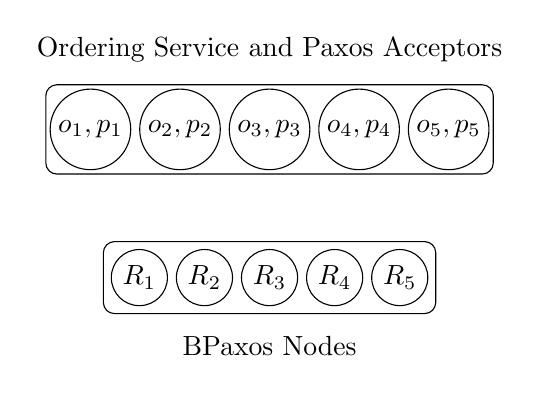
\begin{tikzpicture}
    \tikzstyle{machine}=[draw, circle, inner sep=2pt]

    % Ordering Service / Paxos Acceptors
    \node[machine] (o1) at (0, 2) {$o_1, p_1$};
    \node[machine, right=0.1cm of o1] (o2) {$o_2, p_2$};
    \node[machine, right=0.1cm of o2] (o3) {$o_3, p_3$};
    \node[machine, right=0.1cm of o3] (o4) {$o_4, p_4$};
    \node[machine, right=0.1cm of o4] (o5) {$o_5, p_5$};
    \node (os) at ($(o3.north) + (0, 0.5)$) {Ordering Service and Paxos Acceptors};
    \draw[rounded corners]
      ($(o1.south west) + (-0.2, -0.2)$) rectangle
      ($(o5.north east) + (0.2, 0.2)$);

    % BPaxos Nodes
    \node[machine, below=1cm of o3] (b3) {$R_3$};
    \node[machine, left=0.1cm of b3] (b2) {$R_2$};
    \node[machine, left=0.1cm of b2] (b1) {$R_1$};
    \node[machine, right=0.1cm of b3] (b4) {$R_4$};
    \node[machine, right=0.1cm of b4] (b5) {$R_5$};
    \draw[rounded corners]
      ($(b1.south west) + (-0.2, -0.2)$) rectangle
      ($(b5.north east) + (0.2, 0.2)$);
      \node (bpaxos) at ($(b3.south) + (0, -0.5)$) {BPaxos Nodes};
  \end{tikzpicture}

  \caption{Colocated BPaxos}\figlabel{ColocatedBPaxos}
\end{figure}
}

Second, we implement our consensus service using Fast Paxos instead of regular
Paxos. We let ballot $0$ be a fast ballot and every other ballot be a classic
ballot. As before, every BPaxos instance $R$ runs phase 1 of Fast Paxos for
every instance $R.i$. In the normal case, $R$ finishes executing phase 1 and
sends phase 2a ``any'' messages to the Fast Paxos acceptors. At this point, the
acceptors are free to vote for the first proposal that they hear from anyone
(not just from $R$).

As before, when a BPaxos node $R$ receives a command $a$ from a client, it
sends the command to the ordering service nodes in some instance $R.i$. Upon
receiving $a$, an ordering service node $o_j$ computes its reply $(a, R.i,
\deps{a}_j)$. Unlike with BPaxos, $o_j$ does not return the reply $(a, R.i,
\deps{a}_j)$ directly to $R$. Instead, it proposes the value $(a, \deps{a}_j)$
in instance $R.i$ to $p_j$ (the colocated Fast Paxos acceptor). As we just
described, $p_j$ votes for the first proposal that it hears from anyone, so
$p_j$ votes for the value $(a, \deps{a}_j)$ in instance $R.i$ and relays its
phase 2b vote back to $R$.

If $R$ receives a superquorum (i.e.\ $f + \floor{\frac{f+1}{2}} + 1$) of phase
2b votes for the same value $(a, \deps{a}_{j_1}) = \cdots = (a,
\deps{a}_{j_{m}})$ in instance $R.i$, then Fast Paxos (and hence BPaxos)
considers the value chosen. Thus, in the best case, BPaxos can commit a value
in one round trip to a superquorum (just like EPaxos).

If $R$ does \emph{not} receive a superquorum of phase 2b votes for the same
value, then it is unsure whether or not a value was chosen and begins
\defword{recovery} for instance $R.i$. We'll explain recovery in one moment. At
any point in time, any other BPaxos node $Q$ may also begin recovery for
instance $R.i$. In practice, a BPaxos node will only begin recovery if it
believes $R$ has failed, but any node may attempt to recover any instance at
any time.

In this incorrect BPaxos variant, the recovery of instance $R.i$ by node $Q$ is
simply the process of $Q$ attempting to get a value chosen in $R.i$ with a
higher ballot. In particular, $Q$ runs Fast Paxos, as described in
\secref{FastPaxos}. If $Q$ reaches phase 3 of Fast Paxos, it proposes a special
$\noop$ command, a command that does not affect the state machine and does not
conflict with any other command.

\paragraph{Incorrectness}
Now, we explore why this variant of BPaxos is incorrect. Assume we are running
this BPaxos variant with $f = 2$, and imagine EPaxos node $Q$ is attempting to
recovery instance $R.i$. $Q$ begins Fast Paxos with ballot 1 and sends phase 1a
messages to some majority of consensus nodes. $Q$ receives the following phase
1b messages from a majority of acceptors:
\begin{itemize}
  \item
    $p_3$ voted for $(a, \set{b})$ in round $0$.
  \item
    $p_4$ voted for $(a, \set{b})$ in round $0$.
  \item
    $p_4$ voted for $(a, \set{c})$ in round $0$.
\end{itemize}

$Q$ then begins phase 2 of Fast Paxos. $p_3$ and $p_4$ voted for the value $(a,
\set{b})$ in round $0$. $p_1$ and $p_2$ maybe also voted for $(a, \set{b})$ in
round $0$, which means that $(a, \set{b})$ may have been chosen in round $0$.
Thus, $Q$ executes Case 2 and proposes that the value $(a, \set{b})$ be chosen.

This is incorrect! It's possible that $p_1$ and $p_2$ did \emph{not} vote for
$(a, \set{b})$ in round $0$. For example, they could have voted for $(a,
\set{c})$. In this case, $\set{b}$, the dependencies proposed by $Q$, are not
the union of responses from a majority of ordering service nodes. This violates
one of the key invariants of BPaxos. The only values that can be proposed to
the consensus service are responses from the ordering service, and $\set{b}$
may not be a response from the ordering service.

More concretely, we can construct the following execution of this incorrect
BPaxos variant in which two conflicting commands are both chosen and neither
depends on the other. $R$ receives command $a$ and $Q$ receives command $b$.
$o_1$ and $o_2$ receive $a$ and propose $(a, \emptyset)$ in instance $R.i$ to
acceptors $p_1$ and $p_2$. Similar, $o_4$ and $o_5$ receive $b$ and propose
$(b, \emptyset)$ in instance $Q.j$ to acceptors $p_4$ and $p_5$. Then, $R$ and
$Q$ crash and all other messages are dropped. Another BPaxos node $S$ attempts
to recover $R.i$. In phase 1 of Fast Paxos, it hears from $p_1$, $p_2$, and
$p_3$, and then gets the value $(a, \emptyset)$ chosen. Then, another node $T$
recovers $Q.j$. In phase 1 of Fast Paxos, it hears from $p_3$, $p_4$, and $p_5$
and then gets the value $(b, \emptyset)$ chosen. $S$ executes $a$ and $T$
executes $b$. If these two commands conflict, this violates execution
consistency.

Taking a step back, we see that the bug with this BPaxos variant arises because
of a mismatch between what BPaxos expects and what Fast Paxos expects. BPaxos
wants to get values of the form $(a, \deps{a})$ chosen, but only if $\deps{a}$
is the union of responses from a majority of ordering service nodes. This is
required to ensure that conflicting commands will depend on one another.
However Fast Paxos wants to get \emph{any} value chosen. Fast Paxos has no
understanding of the ordering service nodes, or any notion that some specific
values should not be chosen. Fast Paxos tries to get any proposed value chosen.
In our example above, when node $S$ received 2 votes for $(a, \emptyset)$ in
round 0, Fast Paxos determined that this value may have been chosen in round 0,
so it happily proposes it. Fast Paxos doesn't understand the additional
requirement that BPaxos requires: that $(a, \emptyset)$ cannot be chosen unless
a majority of ordering service nodes determined that $a$'s dependencies should
be the empty set.

Here's another way to interpret the incorrectness of this BPaxos variant. When
a node $Q$ is recovering an instance $R.i$ and wants to propose a value $v =
(a, \deps{a})$, it has to perform the logic illustrated in
\figref{BPaxosLogic}.
%
If it's possible that a value $v$ was previously chosen, then to avoid choosing
two different values, we have no choice but to propose $v$.
%
Similarly, if $v$ is a union of responses from a majority of ordering service
nodes, then we're free to propose it, but if $v$ is not the union of responses
from a majority of ordering service nodes, then we can't propose it.
%
If a recovering node $Q$ has a value $v$ that may have been chosen \emph{and}
is maybe not a union of responses from a majority of ordering service nodes,
then $Q$ is stuck. It simultaneously has to propose $v$ and cannot propose $v$.
This is exactly the situation in which our BPaxos variant is incorrect. When
faced with such a value $v$, it erroneously proposes $v$.

\begin{figure}[h]
  \centering
  \begin{tabular}{rccc}
    %
    &
    &
    \multicolumn{2}{p{3in}}{%
      Is $v$ a union of responses from a majority of ordering service nodes?%
    } \\
    %
    &
    &
    yes &
    maybe not \\\cline{3-4}
    %
    \multirow{2}{1.8in}{Was $v$ previously chosen?} &
    maybe &
    \multicolumn{1}{|c|}{Propose it} &
    \multicolumn{1}{|c|}{We're stuck!} \\\cline{3-4}
    %
    &
    definitely not &
    \multicolumn{1}{|c|}{Propose it, or propose noop} &
    \multicolumn{1}{|c|}{Propose noop} \\\cline{3-4}
  \end{tabular}
  \caption{The logic that any BPaxos variant should follow}%
  \figlabel{BPaxosLogic}
\end{figure}

Thus, in order for a BPaxos variant to be correct, it has to eliminate the
possibility that a value $v$ may have been chosen and simultaneously may not be
a union of responses from a majority of ordering service nodes. In the next
couple of sections, we'll introduce a couple of BPaxos variants. We'll see that
each variant uses different mechanisms to ensure that this situation is
impossible.

\section{Unanimous Bipartisan Paxos}\seclabel{UnanimousBPaxos}
TODO: rewrite section.

To prove that this tweak is correct, we have to prove that \emph{every}
execution of our tweaked protocol is identical to \emph{some} execution of our
untweaked protocol. In particular, we have to prove that if our tweaked
protocol gets some value $(x, \deps{x})$ chosen, then it's possible that our
untweaked protocol could have as well. That is, we have to prove that if $(x,
\deps{x})$ is chosen, then $\deps{x}$ is the union of some quorum of ordering
service responses.

To prove this, we begin by proving the claim $P(i)$ that says if an acceptor
votes for value $(x, \deps{x})$ in round $i$, then either
\begin{itemize}
  \item $i = 0$, or
  \item $\deps{x}$ is the union of a quorum of ordering service replies, or
  \item $x$ is a $\noop$ and $\deps{x} = \emptyset{}$.
\end{itemize}
We prove this by induction. $P(0)$ is trivial. For the general case, we perform
a case analysis on the proposer's logic.
\begin{itemize}
  \item (Case 1)
    $V = \set{(x, \deps{x})}$ and $k \neq 0$. $P(i)$ holds directly from
    $P(k)$.

  \item (Case 2)
    If $k \neq 0$, then $P(i)$ holds directly from $P(k)$. If $k = 0$, then
    it's possible that value $(x, \deps{x})$ was chosen in round $0$ only if
    the proposer receives phase 1b messages from a quorum of acceptors such
    that every acceptor voted for $(x, \deps{x})$ (because superquourum sizes
    are $n$). In this case, the value $(x, \deps{x})$ was an ordering service
    reply on at least a majority of nodes, so $P(i)$ holds.

  \item (Case 3)
    In this case, a proposer always chooses to propose a $\noop$, so $P(i)$
    holds trivially.
\end{itemize}

This claim tells us that if any value is chosen in round $i > 0$, then it is
the union of a quorum of ordering service replies or is a $\noop$. In either
case, this execution is possible in the untweaked algorithm. If a value $(x,
\deps{x})$ is chosen in round $0$, then all ordering service nodes replied with
$\deps{x}$, so it is a union of a majority of ordering service replies.

\subsection{Tweak 3: Coordinated Recovery}
After the previous tweak, a BPaxos node $R$ can commit a command in one round
trip if a superquorum of Paxos acceptors happen to vote for the same set of
dependencies. If $R$ does not receive a superquorum of matching votes, it
performs two additional phases of Paxos to get the command chosen in ballot 1.
Thus, we have one round trip commit latency in the best case and three round
trip commit latency in the next best case (and potentially infinitely more
round trips in the worst case~\cite{fischer1982impossibility}). This tweak, the
final tweak, improves BPaxos to one round trip commit latency in the best case
and two round trip commit latency in the next best case. This matches EPaxos'
commit latencies, save that BPaxos' superquorum sizes are one node larger.

The idea behind this tweak is to leverage a Fast Paxos feature called
coordinated recovery. Coordinated recovery says that if a Fast Paxos leader
owns consecutive ballots $i$ and $i + 1$, and hears phase 2b votes from a
quorum of acceptors for ballot $i$, it can skip phase 1 of ballot $i + 1$ and
proceed directly to phase 2. With this tweak, we make each BPaxos node the
leader of ballots $0$ and $1$. If BPaxos node $R$ receives a quorum of
non-equal votes in ballot $0$, it satisfies the conditions of coordinated
recovery and can initiate phase 2 of ballot 1 directly.

This tweak doesn't affect the correctness of BPaxos because it's merely a
performance optimization for Fast Paxos. The correctness of our protocol does
not depend on whether we use Paxos, Fast Paxos, or Fast Paxos with coordinated
recovery to implement our coordination service.

\section{Fast Bipartisan Paxos}
\section{Faster Bipartisan Paxos}

\bibliographystyle{plain}
\bibliography{references}

\begin{appendices}

  \section{An Aside on Fast Paxos}\seclabel{FastPaxos}
Before we move on, we summarize the relevant bits of Fast
Paxos~\cite{lamport2006fast} that are critical to our remaining BPaxos
variants. In Fast Paxos, after a proposer receives phase 1b messages from a
quorum of acceptors, it performs the following logic to select a value to
propose:
\begin{itemize}
  \item
    Let $k$ be the largest vote round in the quorum of phase 1b messages.
    Let $V$ be the corresponding set of vote values for round $k$.
  \item
    (Case 1) If $V = \set{v}$, then propose $v$.
  \item
    (Case 2) If $V$ contains a value $v$ that may have been chosen in round
    $k$, propose $v$. Note that quorum sizes are selected in such a way that at
    most one such $v$ can exist.
  \item
    (Case 3) Otherwise, propose anything.
\end{itemize}

Proving the correctness of Fast Paxos involves proving the statement $P(i)$
that says that if an acceptor votes for a value $v$ in round $i$, then no
other value besides $v$ has been or will be chosen in any round $j$ less than
$i$. We prove this claim by induction. $P(0)$ is trivial because there are no
rounds less than $0$. For the general case, we perform a case analysis on $j$.
First, assume $k \neq -1$.
\begin{itemize}
  \item
    If $k < j < i$, then no value has been or will be chosen in round $j$
    because a phase 1 quorum of acceptors had not voted in any round larger
    than $k$ and promised not to vote in any round less than $i$.

  \item
    If $k = j$, then we perform a case analysis on the proposer's logic.
    \begin{itemize}
      \item
        (Case 1) If $V = \set{v}$, then a quorum of acceptors have either voted
        for $v$ in round $k$ or promised not to vote in round $k$. Thus, no
        other value besides $v$ can be chosen in round $k$.
      \item
        (Case 2) If $V$ contains a value that may have been chosen in round
        $k$, we propose it. Quorum sizes are set up such that no other value
        could have been chosen in round $k$.
      \item
        (Case 3) No value could have been chosen in round $k$.
    \end{itemize}

  \item
    If $j < k$, we again perform a case analysis on the proposer's logic.
    \begin{itemize}
      \item
        (Case 1) By $P(k)$, no value other than $v$ has been or will be chosen
        in round $j$.
      \item
        (Case 2) Let $v_1, v_2 \in V$. By $P(v_1), P(v_2)$, no value has been
        or will be chosen in round $j$.
      \item
        (Case 3) Same as Case 2.
    \end{itemize}
\end{itemize}
If $k = -1$, then we know that no value has been or will be chosen in any round
less than $i$ by the same line of reasoning as above, so we're free to propose
anything.

Note that we can make the following small tweak to Fast Paxos without
compromising its correctness. We can change Case 1 of the proposer's logic from
``If $V = \set{v}$, then propose $v$'' to ``If $V = \set{v}$ and $k \neq 0$,
then propose $v$''. That is, a proposer will only perform Case 1 if $k \neq 0$.

\end{appendices}
\end{document}
